\chapter{E-pH-diagrammen}\label{ch:b1:e-ph-diagrams}

Een ijzeren spijker in regenwater roest; dezelfde spijker in een sterk
basische oplossing blijft wekenlang blinken. De stalen romp van een schip
draagt blokken zink die in zijn plaats oplossen, en een koperen dak wordt
groen maar verdwijnt nooit. \omterm{def:b1:nernst:couple}{Redoxkoppels} waarvan de potentiaal van de pH
afhangt, neerslagvorming van hydroxiden en oxiden, zuur-base-evenwichten:
alle drie werken tegelijk, en één enkele kaart brengt ze samen. Op een
grafiek van de potentiaal tegen de pH krijgt elk deeltje van een element
het gebied waar het de stabiele vorm is; het lezen van de kaart zegt
welke deeltjes in water overleven, welke met elkaar reageren, en waar
een metaal corrodeert.

\begin{recall}
De \omterm{thm:b1:nernst:nernst}{vergelijking van Nernst}, de \omterm{def:b1:nernst:electrode-potential}{standaardpotentialen} en het voorspellen van
redoxreacties staan in \cref{ch:b1:nernst}; \omterm{def:b1:predominant-reaction:predominance}{predominantiediagrammen} in
\cref{ch:b1:predominant-reaction}; neerslagdrempels van hydroxiden en
\omterm{def:b1:precipitation:existence-domain}{existentiegebieden} van vaste stoffen in \cref{ch:b1:precipitation}. Alle
potentialen gelden bij \qty{25}{\celsius}, met
$RT\ln 10/F = \qty{0.059}{V}$.
\end{recall}

\begin{omfigure}
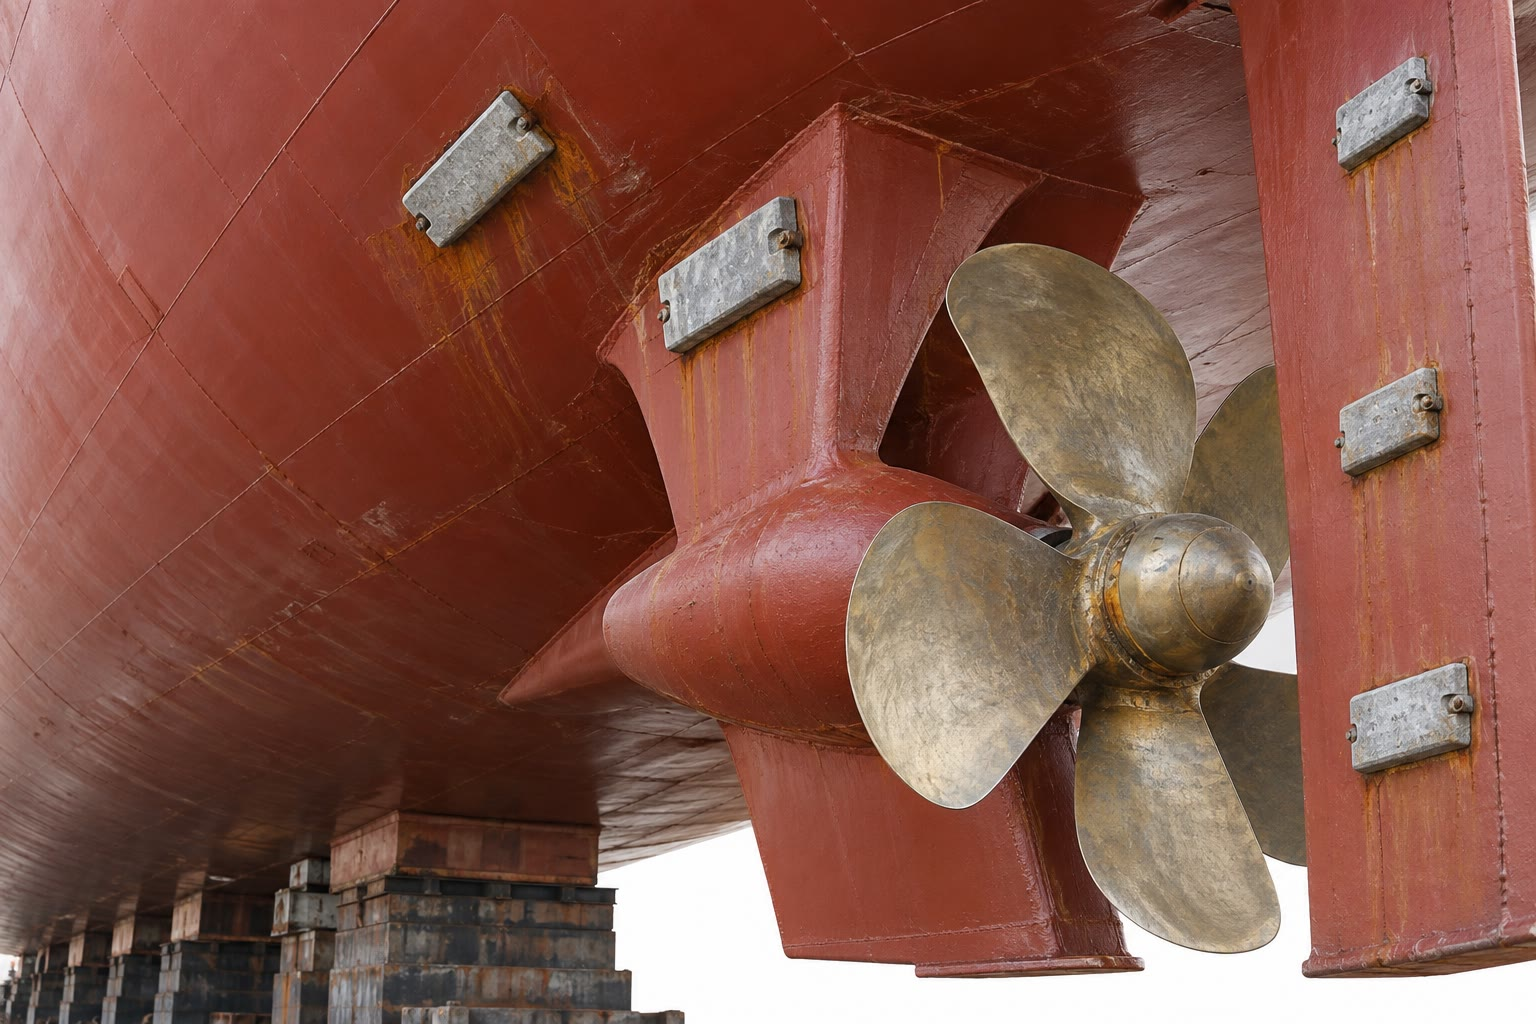
\includegraphics[width=0.6\linewidth]{images/book2/ai/b1-14-ship-anodes.jpg}

{\small De achtersteven van een schip in het droogdok. De grijze blokken
die bij de schroef aan de romp bevestigd zijn, zijn van zink: in zeewater
corroderen zij in plaats van het staal (\cref{exo:b1:e-ph-diagrams:12}).}
\end{omfigure}

\section{Afspraken}

\begin{definition}[Potentiaal-pH-diagram, werkconcentratie]\label{def:b1:e-ph-diagrams:e-ph-diagram}
Het \emph{potentiaal-pH-diagram}\index{potentiaal-pH-diagram} van een
element is het vlak $(\mathrm{pH}, E)$, verdeeld in gebieden die elk het
predominantiegebied (opgeloste deeltjes) of het \omterm{def:b1:precipitation:existence-domain}{existentiegebied} (vaste
stoffen) van één vorm van het element zijn. Het wordt getekend voor een
gekozen \emph{werkconcentratie}\index{werkconcentratie} $c$, de totale
concentratie van het element in oplossing, met de volgende afspraken:
\begin{itemize}
  \item op een grens tussen twee opgeloste deeltjes is elk ervan op $c$
        (geteld in atomen van het element);
  \item op een grens tussen een opgelost deeltje en een vaste stof is het
        opgeloste deeltje op $c$ en is de vaste stof net aanwezig;
  \item gassen staan onder \qty{1}{bar}.
\end{itemize}
In dit hoofdstuk is $c = \qty{0.010}{mol/L}$.
\end{definition}

De vormen van het element worden gerangschikt naar \omterm{def:b1:nernst:oxidation-number}{oxidatiegetal}: hoe
hoger het getal, hoe hoger in het diagram (geoxideerde vormen zijn
stabiel bij hoge potentiaal). Bij een gegeven \omterm{def:b1:nernst:oxidation-number}{oxidatiegetal} liggen de
meer basische vormen (hydroxiden, oxiden, hydroxocomplexen) rechts.

\begin{proposition}[Helling van een grens]\label{prop:b1:e-ph-diagrams:boundary-slope}
Een grens tussen twee deeltjes met verschillende \omterm{def:b1:nernst:oxidation-number}{oxidatiegetallen}, waarvan
de \omterm{def:b1:nernst:couple}{halfreactie} $n$ elektronen en $m$ protonen uitwisselt,
$\mathrm{Ox} + m\,\ce{H+} + n\,\mathrm{e^-} \rightleftharpoons \mathrm{Red} +
\cdots$, is een rechte met helling $-0.059\,m/n$ volt per pH-eenheid. Een
grens tussen twee deeltjes met hetzelfde \omterm{def:b1:nernst:oxidation-number}{oxidatiegetal} is verticaal.
\end{proposition}

\begin{proof}
De \omterm{thm:b1:nernst:nernst}{vergelijking van Nernst} geeft $E = E^\circ + \frac{0.059}{n}\log\frac{[\mathrm{Ox}]
[\ce{H+}]^m}{[\mathrm{Red}]} = E^\circ + \frac{0.059}{n}\log\frac{[\mathrm{Ox}]}
{[\mathrm{Red}]} - \frac{0.059\,m}{n}\,\mathrm{pH}$, en op de grens liggen
de concentraties vast door de afspraken. Twee deeltjes met hetzelfde
\omterm{def:b1:nernst:oxidation-number}{oxidatiegetal} zijn verbonden door een zuur-base- of neerslagevenwicht
zonder elektronen, waarvan de constante de pH van de grens vastlegt, wat
de potentiaal ook is.
\end{proof}

\section{Water}

\begin{proposition}[De twee lijnen van water]\label{prop:b1:e-ph-diagrams:water-lines}
Onder \qty{1}{bar} gas wordt water gereduceerd tot waterstof onder de
lijn $E = -0.059\,\mathrm{pH}$ en geoxideerd tot zuurstof boven de lijn
$E = 1.23
- 0.059\,\mathrm{pH}$.
\end{proposition}

\begin{proof}
\ce{2H+ + 2e- -> H2}: $E = 0 + \frac{0.059}{2}\log\frac{[\ce{H+}]^2}{p(\ce{H2})}
= -0.059\,\mathrm{pH}$ bij $p = 1$. \ce{O2 + 4H+ + 4e- -> 2H2O}: $E = 1.23 +
\frac{0.059}{4}\log(p(\ce{O2})[\ce{H+}]^4) = 1.23 - 0.059\,\mathrm{pH}$.
Onder de eerste lijn is \ce{H2} de stabiele vorm van het koppel (water
wordt gereduceerd); boven de tweede is dat \ce{O2}.
\end{proof}

\begin{definition}[Stabiliteitsgebied van water]\label{def:b1:e-ph-diagrams:water-domain}
De band tussen de twee lijnen, bij elke pH \qty{1.23}{V} breed, is het
\emph{stabiliteitsgebied van water}\index{stabiliteitsgebied van water}:
een deeltje waarvan het gebied er volledig binnen ligt, oxideert noch
reduceert water.
\end{definition}

\section{Een diagram opbouwen: ijzer}

\begin{method}[Een potentiaal-pH-diagram opbouwen]\label{met:b1:e-ph-diagrams:build}
\begin{enumerate}
  \item Som de deeltjes op en rangschik ze naar \omterm{def:b1:nernst:oxidation-number}{oxidatiegetal}: voor
        ijzer \ce{Fe} (0), \ce{Fe^2+} en \ce{Fe(OH)2} ($+$II), \ce{Fe^3+}
        en \ce{Fe(OH)3} ($+$III).
  \item Bepaal bij elk \omterm{def:b1:nernst:oxidation-number}{oxidatiegetal} de verticale grenzen uit de neerslag-
        (of zuur-base-)evenwichten bij de \omterm{def:b1:e-ph-diagrams:e-ph-diagram}{werkconcentratie}
        (\cref{ch:b1:precipitation}).
  \item Schrijf voor elk paar naburige \omterm{def:b1:nernst:oxidation-number}{oxidatiegetallen} in elk pH-gebied
        de \omterm{def:b1:nernst:couple}{halfreactie} op en haar \omterm{thm:b1:nernst:nernst}{vergelijking van Nernst} met de
        afspraken; dat geeft een rechte grens met bekende helling.
  \item Zet de lijnen van links naar rechts aan elkaar; waar drie lijnen
        samenkomen, loopt elke lijn alleen door aan de kant waar haar twee
        deeltjes allebei stabiel zijn.
  \item Controleer: de gebieden mogen niet overlappen, en de hellingen
        moeten overeenstemmen met \cref{prop:b1:e-ph-diagrams:boundary-slope}.
\end{enumerate}
\end{method}

\begin{example}[De grenzen van ijzer]\label{ex:b1:e-ph-diagrams:iron}
Met $c = \qty{0.010}{mol/L}$ (en de constanten van \cref{ch:b1:precipitation,ch:b1:nernst}):
\begin{itemize}
  \item \ce{Fe^3+}/\ce{Fe(OH)3}: $\mathrm{pH} = 14.00 - \frac13(38.55 - 2) = 1.82$;
        \ce{Fe^2+}/\ce{Fe(OH)2}: $\mathrm{pH} = 14.00 - \frac12(16.31 - 2) = 6.85$.
  \item \ce{Fe^2+}/\ce{Fe}: $E = -0.41 + 0.030\log c = -0.47$~V (pH onder
        6.85).
  \item \ce{Fe^3+}/\ce{Fe^2+}: $E = 0.77$~V (beide op $c$, pH onder 1.82).
  \item \ce{Fe(OH)3}/\ce{Fe^2+}: \ce{Fe(OH)3 + 3H+ + e- -> Fe^2+ + 3H2O},
        helling
        $-0.177$: $E = 1.09 - 0.177\,\mathrm{pH}$ tussen pH 1.82 en 6.85.
  \item \ce{Fe(OH)3}/\ce{Fe(OH)2}: één elektron, één proton, $E = 0.28 -
        0.059\,\mathrm{pH}$; \ce{Fe(OH)2}/\ce{Fe}: twee elektronen, twee
        protonen, $E = -0.07 - 0.059\,\mathrm{pH}$ (pH boven 6.85).
\end{itemize}
De ordinaten bij de oorsprong volgen uit de continuïteit in de
tripelpunten, of rechtstreeks uit de vormingsenergieën van Gibbs; het
diagram hieronder is met die laatste berekend, en zijn grenzen
verschillen minder dan \qty{0.01}{V} of 0.01 pH-eenheid van deze
afgeronde waarden.
% ledger: dfg:Fe2+_ao, dfg:Fe3+_ao, dfg:Fe_OH2_cr, dfg:Fe_OH3_cr, dfg:H2O_l, dfg:OH-_ao (boundaries computed in figdata/bachelor-1/eph-diagrams.py)
\end{example}

\begin{omfigure}
\begin{tikzpicture}
\begin{axis}[
  width=0.8\linewidth, height=8.2cm, xmin=0, xmax=14, ymin=-1.2, ymax=1.6,
  axis x line=bottom, axis y line=left, xlabel={pH}, ylabel={$E$ (V)},
  xtick={0,2,4,6,8,10,12,14}, ytick={-1,-0.5,0,0.5,1,1.5},
  unbounded coords=jump, clip=true,
  tick label style={font=\small}, label style={font=\small}]
\addplot[black!45, dashed] table[x=pH, y=H2] {figdata/out/bachelor-1-eph-diagrams-water.dat};
\addplot[black!45, dashed] table[x=pH, y=O2] {figdata/out/bachelor-1-eph-diagrams-water.dat};
\addplot[omDef, very thick] table[x=pH, y=E] {figdata/out/bachelor-1-eph-diagrams-iron.dat};
\node[font=\small] at (axis cs:3.2,-0.85) {\ce{Fe}};
\node[font=\small] at (axis cs:3.4,0.15) {\ce{Fe^2+}};
\node[font=\small] at (axis cs:0.9,1.45) {\ce{Fe^3+}};
\node[font=\small] at (axis cs:8.5,0.25) {\ce{Fe(OH)3}};
\node[font=\scriptsize] at (axis cs:11.0,-0.56) {\ce{Fe(OH)2}};
\node[font=\scriptsize, black!55, rotate=-14, anchor=south] at (axis cs:12.0,0.52) {\ce{O2}/\ce{H2O}};
\node[font=\scriptsize, black!55, rotate=-14, anchor=south] at (axis cs:2.2,-0.11) {\ce{H2O}/\ce{H2}};
\end{axis}
\end{tikzpicture}

{\small \omterm{def:b1:e-ph-diagrams:e-ph-diagram}{Potentiaal-pH-diagram} van ijzer voor $c = \qty{0.010}{mol/L}$
(volle lijnen), met de twee lijnen van water (gestreept). Elke grens is
berekend uit getabelleerde vormingsenergieën van Gibbs.}
\end{omfigure}

\section{Koper en zink}

Dezelfde methode geeft de diagrammen van koper (deeltjes \ce{Cu}, \ce{Cu+},
\ce{Cu2O} bij $+$I, \ce{Cu^2+}, \ce{CuO} bij $+$II) en van zink (\ce{Zn},
\ce{Zn^2+}, \ce{Zn(OH)2}, \ce{Zn(OH)4^2-}). Voor koper verschijnt
\ce{CuO} bij $\mathrm{pH} = 14.00 - \frac12(20.64 - 2) = 4.68$, en het
\ce{Cu+}-ion heeft, hoewel het opgesomd is, helemaal geen gebied: in zuur
milieu ligt $E^\circ(\ce{Cu+}/\ce{Cu}) = 0.52$~V boven
$E^\circ(\ce{Cu^2+}/\ce{Cu+}) = 0.16$~V, zodat zijn vermeende gebied door
de twee buren weggestreept wordt (\cref{sec:b1:e-ph-diagrams:reading}).
Voor zink verschijnt het hydroxide bij pH 6.81 en lost het bij deze
concentratie pas boven 13.97 weer op als \ce{Zn(OH)4^2-}, een smalle
strook aan de rechterrand.

\begin{omfigure}
\begin{tikzpicture}
\begin{axis}[name=cu,
  width=0.47\linewidth, height=7cm, xmin=0, xmax=14, ymin=-1.4, ymax=1.6,
  axis x line=bottom, axis y line=left, xlabel={pH}, ylabel={$E$ (V)},
  xtick={0,4,8,12}, ytick={-1,-0.5,0,0.5,1,1.5},
  unbounded coords=jump, clip=true,
  tick label style={font=\small}, label style={font=\small}]
\addplot[black!45, dashed] table[x=pH, y=H2] {figdata/out/bachelor-1-eph-diagrams-water.dat};
\addplot[black!45, dashed] table[x=pH, y=O2] {figdata/out/bachelor-1-eph-diagrams-water.dat};
\addplot[omDef, very thick] table[x=pH, y=E] {figdata/out/bachelor-1-eph-diagrams-copper.dat};
\node[font=\small] at (axis cs:5,-0.7) {\ce{Cu}};
\node[font=\small] at (axis cs:2,0.7) {\ce{Cu^2+}};
\node[font=\small] at (axis cs:9.5,0.75) {\ce{CuO}};
\node[font=\scriptsize] (cuo) at (axis cs:11.8,-1.05) {\ce{Cu2O}};
\draw[->, black!70] (cuo.north) -- (axis cs:10,-0.035);
\node[font=\small, anchor=north] at (axis cs:7,1.58) {koper};
\end{axis}
\begin{axis}[at={(cu.east)}, anchor=west, xshift=1.5cm,
  width=0.47\linewidth, height=7cm, xmin=0, xmax=14, ymin=-1.4, ymax=1.6,
  axis x line=bottom, axis y line=left, xlabel={pH}, ylabel={$E$ (V)},
  xtick={0,4,8,12}, ytick={-1,-0.5,0,0.5,1,1.5},
  unbounded coords=jump, clip=true,
  tick label style={font=\small}, label style={font=\small}]
\addplot[black!45, dashed] table[x=pH, y=H2] {figdata/out/bachelor-1-eph-diagrams-water.dat};
\addplot[black!45, dashed] table[x=pH, y=O2] {figdata/out/bachelor-1-eph-diagrams-water.dat};
\addplot[omDef, very thick] table[x=pH, y=E] {figdata/out/bachelor-1-eph-diagrams-zinc.dat};
\node[font=\small] at (axis cs:3.5,-1.15) {\ce{Zn}};
\node[font=\small] at (axis cs:3.2,0.4) {\ce{Zn^2+}};
\node[font=\small] at (axis cs:10.2,0.4) {\ce{Zn(OH)2}};
\draw[->] (axis cs:12.4,1.15) node[left, font=\scriptsize] {\ce{Zn(OH)4^2-}} -- (axis cs:13.95,1.15);
\node[font=\small, anchor=north] at (axis cs:10.5,1.58) {zink};
\end{axis}
\end{tikzpicture}

{\small \omterm{def:b1:e-ph-diagrams:e-ph-diagram}{Potentiaal-pH-diagrammen} van koper en zink ($c =
\qty{0.010}{mol/L}$), met de lijnen van water (gestreept). Het gebied van
metallisch koper overlapt met het gebied van water; dat van zink ligt
volledig onder de waterstoflijn.}
% ledger: dfg:Cu+_ao, dfg:Cu2+_ao, dfg:Cu2O_cr, dfg:CuO_cr, dfg:Zn2+_ao, dfg:Zn_OH2_cr, dfg:Zn_OH42-_ao (boundaries computed in figdata/bachelor-1/eph-diagrams.py)
\end{omfigure}


\section{Een diagram lezen}\label{sec:b1:e-ph-diagrams:reading}

\begin{proposition}[Disjuncte gebieden]\label{prop:b1:e-ph-diagrams:disjoint-domains}
Als bij een gegeven pH het gebied van een \omterm{def:b1:nernst:couple}{oxidator} volledig boven dat van
een \omterm{def:b1:nernst:couple}{reductor} ligt, zonder gemeenschappelijk deel, reageren de twee;
deeltjes waarvan de gebieden een gebied gemeen hebben, kunnen in
evenwicht naast elkaar bestaan.
\end{proposition}

\begin{proof}
Bij die pH heeft het koppel van de \omterm{def:b1:nernst:couple}{oxidator} boven zijn grens een
potentiaal die hoger is dan elke potentiaal die het koppel van de
\omterm{def:b1:nernst:couple}{reductor} kan bereiken: volgens
\cref{prop:b1:nernst:equilibrium-constant} heeft de reactie tussen hen
$K > 1$, en ze gaat door tot een van beide op is of hun gebieden elkaar
raken. Binnen een gemeenschappelijk gebied zijn beide de stabiele vormen
bij dezelfde potentiaal: niets drijft een reactie aan.
\end{proof}

IJzer en water: het gebied van metallisch ijzer ligt bij elke pH onder de
lijn \ce{H2O}/\ce{H2}. IJzer reduceert water, in zure oplossing met een
zichtbare ontwikkeling van waterstof; met opgeloste zuurstof wordt het
nog sneller geoxideerd. Koper: zijn gebied overlapt met dat van water,
zodat koper water en zuren die zelf geen \omterm{def:b1:nernst:couple}{oxidator} zijn niet reduceert,
maar de zuurstof van de lucht, die erboven ligt, oxideert het langzaam
--- het groene patina van daken is een later product van die oxidatie
met koolstofdioxide en zwavelverbindingen. Een diagram zegt wat mogelijk
is, niet hoe snel: veel reacties die het toelaat zijn traag, een vraag
die in het deel van jaar~2 behandeld wordt.

\begin{definition}[Disproportionering, comproportionering]\label{def:b1:e-ph-diagrams:disproportionation}
\emph{Disproportionering}\index{disproportionering} is de reactie van een
deeltje met zichzelf, waarbij een deel geoxideerd en het andere deel
gereduceerd wordt: \ce{2Cu+ -> Cu^2+ + Cu}. Het omgekeerde, twee deeltjes
van hetzelfde element die er één met een tussenliggend \omterm{def:b1:nernst:oxidation-number}{oxidatiegetal}
geven, is
\emph{comproportionering}\index{comproportionering}:
\ce{2Fe^3+ + Fe -> 3Fe^2+}.
\end{definition}

\begin{proposition}[Criterium voor disproportionering]\label{prop:b1:e-ph-diagrams:disproportionation-criterion}
Een deeltje B met een tussenliggend \omterm{def:b1:nernst:oxidation-number}{oxidatiegetal}, in de koppels A/B en
B/C, disproportioneert als $E(\mathrm{B}/\mathrm{C}) > E(\mathrm{A}/\mathrm{B})$:
het heeft dan geen eigen gebied, en één enkele grens A/C vervangt de
twee.
\end{proposition}

\begin{proof}
B is de \omterm{def:b1:nernst:couple}{oxidator} van B/C en de \omterm{def:b1:nernst:couple}{reductor} van A/B. Ligt het koppel B/C
boven A/B, dan laat de gammaregel (\cref{met:b1:nernst:predict-redox}) B
(\omterm{def:b1:nernst:couple}{oxidator}, bovenste koppel) reageren met B (\omterm{def:b1:nernst:couple}{reductor}, onderste koppel),
wat C en A geeft. Meetkundig zou B alleen stabiel zijn boven
$E(\mathrm{B}/\mathrm{C})$ en onder $E(\mathrm{A}/\mathrm{B})$, een lege
verzameling.
\end{proof}

\begin{definition}[Immuniteits-, corrosie- en passiveringsgebied]\label{def:b1:e-ph-diagrams:corrosion-domains}
In het diagram van een metaal is het gebied van het metaal zelf zijn
\emph{immuniteitsgebied}\index{immuniteitsgebied} (het kan niet
geoxideerd worden); de gebieden van zijn opgeloste ionen vormen het
\emph{corrosiegebied}\index{corrosiegebied}; de gebieden van zijn vaste
oxiden en hydroxiden, die het metaal kunnen bedekken, vormen het
\emph{passiveringsgebied}\index{passiveringsgebied}. Of een laag het
metaal werkelijk beschermt, is een kinetische kwestie, die in het deel
van jaar~2 behandeld wordt.
\end{definition}

\begin{method}[Een diagram lezen]\label{met:b1:e-ph-diagrams:read}
\begin{enumerate}
  \item Leg de lijnen van water erover: een deeltje waarvan het gebied
        buiten de waterband ligt, reageert (thermodynamisch) met water.
  \item Leg voor twee deeltjes van verschillende elementen hun diagrammen
        over elkaar: disjuncte gebieden bij de pH die ertoe doet,
        betekenen een reactie.
  \item Zoek voor een metaal het punt (pH, $E$) van het milieu op:
        immuniteit, corrosie of passivering.
  \item Bedenk dat een diagram voor één \omterm{def:b1:e-ph-diagrams:e-ph-diagram}{werkconcentratie} getekend is; de
        grenzen met opgeloste deeltjes verschuiven met $0.059/n$~V per
        decade concentratie.
\end{enumerate}
\end{method}

Zink beschermt ijzer: in zeewater (pH ongeveer 8) zijn het zink en het
staal van een romp met elkaar in contact; zink, met de lagere
potentiaal, wordt eerst geoxideerd, en de elektronen die het afgeeft,
houden het ijzer in of dicht bij zijn \omterm{def:b1:e-ph-diagrams:corrosion-domains}{immuniteitsgebied}. Het zinkblok
wordt verbruikt en bij elk bezoek aan het droogdok vervangen.

\section{Oefeningen}

\begin{exercise}[$\star$]\label{exo:b1:e-ph-diagrams:1}
Rangschik naar het \omterm{def:b1:nernst:oxidation-number}{oxidatiegetal} van het element de deeltjes \ce{Mn},
\ce{Mn^2+}, \ce{MnO2}, \ce{MnO4-}, \ce{Mn(OH)2}, en \ce{Cl-}, \ce{Cl2},
\ce{HClO}, \ce{ClO-}, \ce{ClO3-}.
\end{exercise}

\begin{exercise}[$\star$]\label{exo:b1:e-ph-diagrams:2}
Geef de helling van de grens voor elke \omterm{def:b1:nernst:couple}{halfreactie}:
\ce{Fe(OH)3 + 3H+ + e- -> Fe^2+ + 3H2O}; \ce{2Cu^2+ + H2O + 2e- -> Cu2O + 2H+};
\ce{MnO4- + 8H+ + 5e- -> Mn^2+ + 4H2O}; \ce{Zn(OH)2 + 2H+ + 2e- -> Zn + 2H2O}.
Waarom heeft een van die grenzen een positieve helling?
\end{exercise}

\begin{exercise}[$\star$]\label{exo:b1:e-ph-diagrams:3}
Bij welke pH gaan de lijnen van water door 0~V en door \qty{0.50}{V}?
Hoe breed is het \omterm{def:b1:e-ph-diagrams:water-domain}{stabiliteitsgebied van water} bij pH 7?
\end{exercise}

\begin{exercise}[$\star$]\label{exo:b1:e-ph-diagrams:4}
Geef met het diagram van ijzer de stabiele vorm van ijzer bij
(pH 1, $E = 1.0$~V), (pH 4, $E = 0$), (pH 10, $E = -0.4$~V) en
(pH 10, $E = 0.5$~V).
\end{exercise}

\begin{exercise}[$\star\star$]\label{exo:b1:e-ph-diagrams:5}
Bereken de grens \ce{Fe^2+}/\ce{Fe} en de verticale grens
\ce{Fe^3+}/\ce{Fe(OH)3} opnieuw voor een \omterm{def:b1:e-ph-diagrams:e-ph-diagram}{werkconcentratie} van
\qty{1.0e-6}{mol/L}, de waarde die gebruikt wordt om corrosie te
bespreken. Welke gebieden worden groter?
\end{exercise}

\begin{exercise}[$\star\star$]\label{exo:b1:e-ph-diagrams:6}
Leid de grens \ce{Fe(OH)3}/\ce{Fe^2+} af: schrijf de \omterm{def:b1:nernst:couple}{halfreactie} op en
haar \omterm{thm:b1:nernst:nernst}{vergelijking van Nernst}, en gebruik de continuïteit bij pH 1.82 om
aan te tonen dat $E = 1.09 -
0.177\,\mathrm{pH}$.
\end{exercise}

\begin{exercise}[$\star\star$]\label{exo:b1:e-ph-diagrams:7}
Toon met de tabel van \omterm{def:b1:nernst:electrode-potential}{standaardpotentialen} aan dat \ce{Cu+} bij pH 0
disproportioneert, en geef de potentiaal van de enige grens
\ce{Cu^2+}/\ce{Cu} bij $c = \qty{0.010}{mol/L}$.
\end{exercise}

\begin{exercise}[$\star\star$]\label{exo:b1:e-ph-diagrams:8}
Lost koper bij pH 0 zonder lucht op in zoutzuur? In salpeterzuur
(koppel \ce{NO3-}/\ce{NO}, $E^\circ = 0.96$~V)? Verantwoord met het
diagram en de potentialen.
\end{exercise}

\begin{exercise}[$\star\star$]\label{exo:b1:e-ph-diagrams:9}
Oplossingen van ijzer(II) die aan de lucht blijven staan, worden
geelbruin. Verklaar met het diagram van ijzer en de lijn
\ce{O2}/\ce{H2O}, en schrijf de reactie bij pH 3 op.
\end{exercise}

\begin{exercise}[$\star\star\star$]\label{exo:b1:e-ph-diagrams:10}
Bouw het diagram van zink op voor $c = \qty{0.010}{mol/L}$: bereken de
verticale grenzen bij pH 6.81 en 13.97, de grens \ce{Zn^2+}/\ce{Zn}, en
de vergelijkingen van \ce{Zn(OH)2}/\ce{Zn} en \ce{Zn(OH)4^2-}/\ce{Zn}.
\end{exercise}

\begin{exercise}[$\star\star\star$]\label{exo:b1:e-ph-diagrams:11}
Leg de diagrammen van ijzer en van water over elkaar en bespreek het lot
van een ijzeren spijker in zuurstofvrij water bij pH 2, bij pH 7 en bij
pH 13. Wat verandert er met opgeloste zuurstof?
\end{exercise}

\begin{exercise}[$\star\star\star$]\label{exo:b1:e-ph-diagrams:12}
Opofferingsanoden. Een stalen romp in zeewater (pH 8) is verbonden met
een zinkblok. Leg met de diagrammen uit welk metaal geoxideerd wordt,
schrijf de reacties met opgeloste zuurstof op, en zeg waarom magnesium
ook zou werken en koper de zaak erger zou maken.
\end{exercise}

\section{Probleem: bleekwater en het zwembad}

\begin{problem}[{Weekendprobleem --- \omterm{def:b1:nernst:oxidation-number}{oxidatiegetallen} van chloor, het
zuur-basepaar HClO/ClO\textsuperscript{$-$}, het \omterm{def:b1:e-ph-diagrams:e-ph-diagram}{potentiaal-pH-diagram}
van chloor, en de pH waarboven opgelost chloor disproportioneert}]
\label{pb:b1:e-ph-diagrams:1}
Bleekwater is een basische oplossing van natriumhypochloriet en
natriumchloride; een zwembad wordt ontsmet door het hypochlorigzuur dat
het bevat, bij een pH die iets boven 7 gehouden wordt. Bleekwater mengen
met een zuur reinigingsmiddel maakt chloorgas vrij. Gegevens bij
\qty{25}{\celsius}: $E^\circ(\ce{Cl2(aq)}/\ce{Cl-})
= 1.396$~V, $E^\circ(\ce{HClO}/\ce{Cl2(aq)}) = 1.594$~V,
$\mathrm{p}K_a(\ce{HClO}/\ce{ClO-}) = 7.55$, $RT\ln 10/F = 0.0592$~V;
\omterm{def:b1:e-ph-diagrams:e-ph-diagram}{werkconcentratie} $c = \qty{0.010}{mol/L}$ aan chlooratomen.

\medskip
\noindent\textbf{Deel I --- De deeltjes.}
\begin{enumerate}
  \item Geef het \omterm{def:b1:nernst:oxidation-number}{oxidatiegetal} van chloor in \ce{Cl-}, \ce{Cl2},
        \ce{HClO} en \ce{ClO-}.
  \item Rangschik de vier deeltjes op een verticale as van het
        \omterm{def:b1:nernst:oxidation-number}{oxidatiegetal}.
  \item Welke twee deeltjes hebben hetzelfde \omterm{def:b1:nernst:oxidation-number}{oxidatiegetal}? Hoe zijn ze
        met elkaar verbonden?
  \item Schrijf de \omterm{def:b1:nernst:couple}{halfreactie} op van \ce{Cl2}/\ce{Cl-}.
  \item Schrijf de \omterm{def:b1:nernst:couple}{halfreactie} op van \ce{HClO}/\ce{Cl2}.
  \item Schrijf de \omterm{def:b1:nernst:couple}{halfreactie} op van \ce{ClO-}/\ce{Cl-} in basische
        oplossing.
\end{enumerate}

\medskip
\noindent\textbf{Deel II --- Hypochlorigzuur.}
\begin{enumerate}[resume]
  \item Teken het \omterm{def:b1:predominant-reaction:predominance}{predominantiediagram} van \ce{HClO} en \ce{ClO-} als
        functie van de pH.
  \item Waarom is hun grens in het \omterm{def:b1:e-ph-diagrams:e-ph-diagram}{potentiaal-pH-diagram} verticaal?
  \item Bereken de fractie hypochlorigzuur bij pH 7.4.
  \item Hetzelfde bij pH 8.0. Hypochlorigzuur is het betere
        ontsmettingsmiddel: waarom zorgen zwembadbeheerders ervoor dat de
        pH niet tot 8 oploopt?
  \item Welke vorm is aanwezig in bleekwater (pH ongeveer 12)?
\end{enumerate}

\medskip
\noindent\textbf{Deel III --- Het diagram.}
Met de afspraken van het hoofdstuk staat \ce{Cl2(aq)} op een grens op
$c/2$ en \ce{Cl-}, \ce{HClO}, \ce{ClO-} op $c$.
\begin{enumerate}[resume]
  \item Toon aan dat de grens \ce{Cl2}/\ce{Cl-} ligt bij $E = 1.396 +
        0.0296\log\bigl((c/2)/c^2\bigr) = 1.446$~V, onafhankelijk van de
        pH.
  \item Toon aan dat de grens \ce{HClO}/\ce{Cl2} gegeven wordt door $E = 1.594 -
        0.0296\log 50 - 0.0592\,\mathrm{pH} \approx 1.544 -
        0.0592\,\mathrm{pH}$.
  \item Bepaal de pH waar deze twee lijnen elkaar snijden.
  \item Voorbij die pH is de grens \ce{HClO}/\ce{Cl-}. Schrijf de
        \omterm{def:b1:nernst:couple}{halfreactie} ervan op en toon aan dat de helling $-0.0296$ is.
  \item Bereken $E^\circ(\ce{HClO}/\ce{Cl-})$ uit de twee gegeven
        potentialen.
  \item Schrijf de grens \ce{ClO-}/\ce{Cl-} boven pH 7.55 op; controleer
        de continuïteit ervan bij pH 7.55.
  \item Schets het diagram van pH 0 tot 14, met de lijn \ce{O2}/\ce{H2O}.
  \item Is hypochlorigzuur thermodynamisch stabiel in water? Waarom heeft
        een zwembad toch elke dag maar kleine toevoegingen van chloor
        nodig?
\end{enumerate}

\medskip
\noindent\textbf{Deel IV --- \omterm{def:b1:e-ph-diagrams:disproportionation}{Disproportionering} en het gevaar van zuur.}
\begin{enumerate}[resume]
  \item Wat gebeurt er boven de pH van vraag 14 met opgelost chloor?
        Schrijf de reactie op in water en in basische oplossing.
  \item Hoe wordt bleekwater uit chloor gemaakt?
  \item Schrijf onder dezelfde pH de reactie tussen \ce{HClO} en \ce{Cl-}
        op. Hoe heet ze?
  \item Een zuur toiletreinigingsmiddel brengt bleekwater op pH 1. Wat
        gebeurt er?
  \item Waarom is het gevaar kleiner met een licht zuur product (pH 4)?
        Antwoord met het diagram, en nuanceer daarna.
  \item Geef, op één decimaal, de pH waarboven opgelost chloor bij
        $c = \qty{0.010}{mol/L}$ disproportioneert.
\end{enumerate}
\end{problem}
